\section{Fourier Transforms} \label{sec:fourier}

\subsection{Eigenfunctions and $H(s)$}

An \emph{eigenfunction} $x(t) = e^{j\omega t}$ is a function such that
$S\{x(t)\} = Ax(t)$ for LTI $S$. A property of functions of the form
$e^{j\omega t}$ is that convolution with $h(t)$ yields
\begin{equation}
    x(t) * h(t) = e^{j\omega t} \int_{-\infty}^{\infty} h(\tau) e^{-j\omega \tau} d\tau.
\end{equation}
This is also written as
\begin{equation}
    x(t) * h(t) = e^{j\omega t} \left( |H(j\omega)|e^{j \angle H(j\omega)} \right)
\end{equation}
$H$ is known as the transfer function as has the property that
$Y(S) = H(s)X(s)$, where $Y(s)$ and $X(s)$ are the Laplace transforms
of $y(t)$ and $x(t)$.

\section{Fourier Transform}
Throughout this class we will sometimes see the expression $X(j\omega)$
or $X(e^{j\omega})$.
Note that these are defined as
\begin{equation}
    X(j\omega) = \int_{-\infty}^{\infty} x(t) e^{-j\omega t} dt
\end{equation}
for CT and
\begin{equation}
    X(e^{j\omega}) = \sum_{n=-\infty}^{\infty} x[n] e^{-j\omega n}
\end{equation}
for DT. This transformation is known as the \emph{Fourier Transform}
and works for well-behaved signals.
A signal $x(t)$ is well-behaved iff
\begin{itemize}
    \item $x(t)$ is absolutely integrable over its domain.
    \item $x(t)$ has finite maximum and minimum.
    \item $x(t)$ has finite discontinuities.
\end{itemize}
The original signal can be recovered with
\begin{equation}
    x(t) = \frac{1}{2\pi} \int_{-\infty}^{\infty} X(j\omega) e^{j\omega t} d\omega
\end{equation}
in CT and
\begin{equation}
    x[n] = \frac{1}{2\pi} \int_{-\pi}^{\pi} X(e^{j\omega}) e^{j\omega n} d\omega
\end{equation}
in DT.

If the Fourier series of
\begin{equation}
    x(t) = \sum_{k=-\infty}^{\infty} a_k e^{jk\omega_0 t}
\end{equation}
then the Fourier transform is
\begin{equation}
    X(j\omega) = \sum_{k=-\infty}^{\infty} 2\pi a_k \delta(\omega - k\omega_0).
\end{equation}

This property quickly tells us that the Fourier transform
of $e^{jk\omega_0 t}$ is $2\pi \delta(\omega-k\omega_0)$.
From this the Fourier transforms of sinusoidals quickly follow.

Another important periodic signal is the impulse train,
\begin{equation}
    \sum_{k=-\infty}^{\infty} \delta(t - kT).
\end{equation}
The Fourier series coefficients for
the impulse train are simply $a_k = \frac{1}{T}$,
so the Fourier transform is
$X(j\omega) = \frac{2\pi}{T} \sum_{k=-\infty}^{\infty} \delta(\omega - \frac{2\pi k}{T})$

Note that as $T$ increases, the impulse train gets wider
and wider while its Fourier transform gets narrower and
narrower. This is because, as we will see often, time and
frequency are inversely related. In general, we will find
that
\begin{equation}
    x(at) \leftrightarrow \frac{1}{|a|}X(\frac{j\omega}{a}).
\end{equation}

If $x(t)$ is real, then $|X(j\omega)|$ is even and
$\angle X(j\omega)$ is odd. Moreover, if $x(t)$ is real
and even, then $X(j\omega)$ must be purely real and even,
and if $x(t)$ is real and odd, $X(j\omega)$ is purely
imaginary and odd.

Arguably the most important property we will see is duality.
As an example, a sinc function in time is a rectangular pulse
in frequency, while a rectangular pulse in time is a sinc
function in frequency. Formally,
\begin{equation}
    F\left\{ X(t) \right\} = 2\pi x(-\omega).
\end{equation}

\section{Fourier Transform Properties}

Table \ref{tab:fourier_transform_properties} tabulates
useful properties of Fourier transforms.

\begin{table}[ht]
    \centering
    \caption{Properties of Fourier Transforms}
    \label{tab:fourier_transform_properties}
    \begin{tabular}{llll}
        \toprule
        \textbf{Property}  & \textbf{Time Domain}                &                                          & \textbf{Frequency Domain}                                     \\
        \midrule
        Linearity          & $A x_1(t) + B x_2(t)$               & $\overset{\mathcal{F}}{\leftrightarrow}$ & $A X_1(j\omega) + B X_2(j\omega)$                             \\[1mm]
        Time Shifting      & $x(t - t_0)$                        & $\overset{\mathcal{F}}{\leftrightarrow}$ & $X(j\omega)e^{-j\omega t_0}$                                  \\[1mm]
        Frequency Shifting & $x(t)e^{j\omega_0 t}$               & $\overset{\mathcal{F}}{\leftrightarrow}$ & $X(j(\omega - \omega_0))$                                     \\[1mm]
        Time Scaling       & $x(at)$, $a > 0$                    & $\overset{\mathcal{F}}{\leftrightarrow}$ & $\frac{1}{|a|}X\left(\frac{j\omega}{a}\right)$                \\[1mm]
        Time Reversal      & $x(-t)$                             & $\overset{\mathcal{F}}{\leftrightarrow}$ & $X(-j\omega)$                                                 \\[1mm]
        Conjugation        & $x^*(t)$                            & $\overset{\mathcal{F}}{\leftrightarrow}$ & $X^*(-j\omega)$                                               \\[1mm]
        Differentiation    & $\frac{d^n}{dt^n}x(t)$              & $\overset{\mathcal{F}}{\leftrightarrow}$ & $(j\omega)^n X(j\omega)$                                      \\[1mm]
        Integration        & $\int_{-\infty}^t x(\tau) d\tau$    & $\overset{\mathcal{F}}{\leftrightarrow}$ & $\frac{X(j\omega)}{j\omega} + \pi X(0)\delta(\omega)$         \\[1mm]
        Convolution        & $(x_1 * x_2)(t)$                    & $\overset{\mathcal{F}}{\leftrightarrow}$ & $X_1(j\omega) X_2(j\omega)$                                   \\[1mm]
        Multiplication     & $x_1(t)x_2(t)$                      & $\overset{\mathcal{F}}{\leftrightarrow}$ & $\frac{1}{2\pi}(X_1 * X_2)(j\omega)$                          \\[1mm]
        Parseval's Theorem & $\int_{-\infty}^\infty |x(t)|^2 dt$ & $\overset{\mathcal{F}}{\leftrightarrow}$ & $\frac{1}{2\pi} \int_{-\infty}^\infty |X(j\omega)|^2 d\omega$ \\
        \bottomrule
    \end{tabular}
\end{table}

Table \ref{tab:ctfourier_transforms} tabulates the
Fourier transform of common continuous time functions.

\begin{table}[ht]
    \centering
    \caption{CT Fourier Transforms}
    \label{tab:ctfourier_transforms}
    \begin{tabular}{ll}
        \toprule
        \textbf{Time Domain Function} & \textbf{Fourier Transform}                                                    \\
        \midrule
        $\delta(t)$                   & $1$                                                                           \\[1mm]
        $1$                           & $2\pi\,\delta(\omega)$                                                        \\[1mm]
        $u(t)$                        & $\pi\,\delta(\omega) + \frac{1}{j\omega}$                                     \\[1mm]
        $e^{-at}u(t),\quad \Re(a)>0$  & $\dfrac{1}{a+j\omega}$                                                        \\[1mm]
        $\cos(\omega_0 t)$            & $\pi\Bigl[\delta(\omega-\omega_0) + \delta(\omega+\omega_0)\Bigr]$            \\[1mm]
        $\sin(\omega_0 t)$            & $\dfrac{\pi}{j}\Bigl[\delta(\omega-\omega_0) - \delta(\omega+\omega_0)\Bigr]$ \\[1mm]
        $\mathrm{rect}(t/T)$          & $T\,\mathrm{sinc}\Bigl(\dfrac{\omega T}{2}\Bigr)$                             \\[1mm]
        $e^{-t^2}$                    & $\sqrt{\pi}\,e^{-\omega^2/4}$                                                 \\
        \bottomrule
    \end{tabular}
\end{table}

Table \ref{tab:dtfourier_transforms} tabulates the
Fourier transform of common discrete time functions.

\begin{table}[ht]
    \centering
    \caption{DT Fourier Transforms}
    \label{tab:dtfourier_transforms}
    \begin{tabular}{ll}
        \toprule
        \textbf{Time Domain Function}          & \textbf{Fourier Transform}                                                                                             \\
        \midrule
        $\delta[n]$                            & $1$                                                                                                                    \\[1mm]
        $1$                                    & $2\pi\,\sum_{k=-\infty}^{\infty}\delta(\omega-2\pi k)$                                                                 \\[1mm]
        $a^n u[n],\quad |a|<1$                 & $\dfrac{1}{1-ae^{-j\omega}}$                                                                                           \\[1mm]
        $\cos(\omega_0 n)$                     & $\pi\,\sum_{k=-\infty}^{\infty}\Bigl[\delta(\omega-\omega_0-2\pi k) + \delta(\omega+\omega_0-2\pi k)\Bigr]$            \\[1mm]
        $\sin(\omega_0 n)$                     & $\dfrac{\pi}{j}\,\sum_{k=-\infty}^{\infty}\Bigl[\delta(\omega-\omega_0-2\pi k) - \delta(\omega+\omega_0-2\pi k)\Bigr]$ \\[1mm]
        $\mathrm{rect}\Bigl(\frac{n}{N}\Bigr)$ & $\dfrac{\sin\Bigl(\frac{\omega N}{2}\Bigr)}{\sin\Bigl(\frac{\omega}{2}\Bigr)}\,e^{-j\omega\frac{N-1}{2}}$              \\
        \bottomrule
    \end{tabular}
\end{table}

\subsection{Continuous Time Fourier Series}

Consider an arbitrary periodic CT signal $x(t)$ with fundemental
period $T$ and fundemental frequency $\omega_0$. The Fourier series
representation of $x(t)$ is
\begin{align}\label{eq:synthesis}
    x(t) & = \sum_{k=-\infty}^{\infty} a_k e^{jk\omega_0 t}                                  \\
         & = a_0 + a_1e^{j\omega_0 t} + a_{-1}e^{-j\omega_0 t} + a_2e^{2j\omega_0 t} + \dots
\end{align}
where $a_k$ is the $k$th Fourier coefficient and can be found with the formula
\begin{equation}
    a_k = \frac{1}{T} \int_{<T>} x(t) e^{-jk\omega_0 t} dt
\end{equation}
with $<T>: [0, T], [-\frac{T}{2}, \frac{T}{2}, ...]$.
Equation \ref{eq:synthesis} is known as the synthesis equation. The process of
of finding $a_k$ is Fourier analysis.

Notably, $a_0$ gives the DC component of the signal. In general the $a_{\pm k}$
are the $k$th harmonic components.

Let's see an example. Let $x(t)$ be a square wave given by
\begin{equation}
    x(t) = \begin{cases}
        1 & |t| < T_1               \\
        0 & T_1 < |t| < \frac{T}{2}
    \end{cases}
\end{equation}

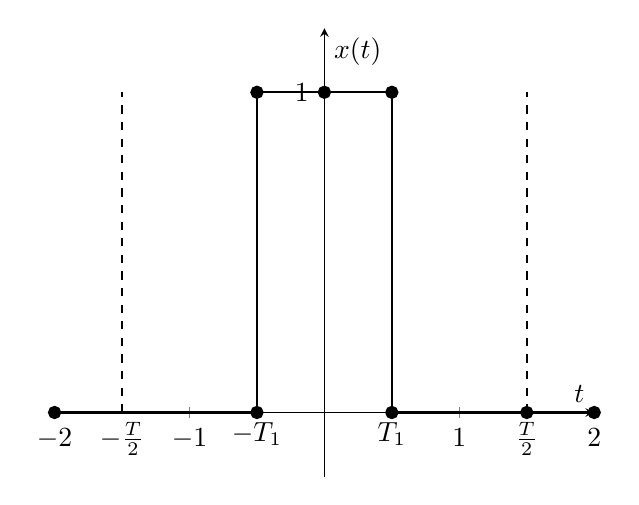
\begin{tikzpicture}
    \begin{axis}[
            axis x line=middle,
            axis y line=middle,
            xlabel={$t$},
            ylabel={$x(t)$},
            xtick={-2, -1, 0, 1, 2},
            ytick={0, 1},
            ymin=-0.2, ymax=1.2,
            xmin=-2, xmax=2,
            samples=100,
            domain=-2:2,
        ]
        \addplot[
            domain=-2:2,
            samples at={-2,-1.5,-1, -0.5, 0, 0.5, 1, 1.5, 2},
            mark=*,
            thick
        ] coordinates {(-2,0) (-0.5,0) (-0.5,1) (0,1) (0.5,1) (0.5,0) (1.5,0) (2,0)};

        \addplot[dashed, thick] coordinates {(-0.5,0) (-0.5,1)};
        \addplot[dashed, thick] coordinates {(0.5,0) (0.5,1)};
        \addplot[dashed, thick] coordinates {(1.5,0) (1.5,1)};
        \addplot[dashed, thick] coordinates {(-1.5,0) (-1.5,1)};

        \node[anchor=north] at (axis cs:-0.5,0) {$-T_1$};
        \node[anchor=north] at (axis cs:0.5,0) {$T_1$};
        \node[anchor=north] at (axis cs:1.5,0) {$\frac{T}{2}$};
        \node[anchor=north] at (axis cs:-1.5,0) {$-\frac{T}{2}$};
    \end{axis}
\end{tikzpicture}

We calculate $a_k$ as
\begin{align}
    a_k & = \frac{1}{T} \int_{<T>} x(t) e^{-jk\omega_0 t} dt                                         \\
        & = -\frac{1}{jk\omega_0 T} \left[ e^{-jk\omega_0 T_1} -  e^{jk\omega_0 T_1}\right]          \\
        & = \frac{1}{k\omega_0 T} \left[ \frac{e^{jk\omega_0 T_1} -  e^{-jk\omega_0 T_1}}{j} \right] \\
        & = \frac{2}{\omega_0 T} \sin(k \omega_0 T_1)                                                \\
        & = \frac{1}{\pi k} \sin(k \omega_0 T_1)
\end{align}
This expression for $a_0$ is fine, however, there is a problem. When
$k = 0$ we have a discontinuity. In general we may have to find $a_0$
separately. It's not a big deal: $a_0 = \frac{1}{T} \int_{-T_1}^{T_1} x(t) dt$ in general`'.

\subsection{Discrete Time Fourier Series}

In discrete time, an arbitrary periodic signal $x[n]$ with fundemental
period $N$ and fundemental frequency $\omega_0$. The Fourier series
representation of $x[n]$ is
\begin{align}\label{eq:dtsynthesis}
    x[n] & = \sum_{k=<N>} a_k x_k[n]           \\
         & = \sum_{k=<N>} a_k e^{jk\omega_0 n}
\end{align}

This expression yields a system of $n$ linear equations with $n$
unknowns, namely $x[0]$, $x[1]$, $\dots$, $x[n]$. In theory we
could solve this, perhaps using computers or linear algebra, but
in practice there is a simpler way. Multiply equation \ref{eq:dtsynthesis}
by $e^{-jr\frac{2\pi}{N}n}$ for any $r$ and sum over $N$ terms. Then
\begin{equation}
    \sum_{n=<N>} x_k[n] e^{-jr\frac{2\pi}{N}n} = \sum_{n=<N>} a_k \sum_{n=<N>} e^{j(k-r)(\frac{2\pi}{N})n}.
\end{equation}
Solving for $a_k$,
\begin{equation}
    a_k = \frac{1}{N} \sum_{n=<N>} x[n] e^{-jk\frac{2\pi}{N}n},
\end{equation}
which is the synthesis equation in discrete time.

A fun property is that $a_{k+N} = a_k$, so $a_k$ are periodic in $N$.

\subsection{Spectrum Analysis}

$a_k$ as a function of $k$ given the \emph{spectrum} of $x(t)$. Let's see
an example: let $T_1 = \frac{T}{4}$. Then $a_k = \frac{\sin(\pi \frac{k}{2})}{k\pi}$.

\begin{tikzpicture}
    \begin{axis}[
            axis x line=middle,
            axis y line=middle,
            xlabel={$t$},
            ylabel={$x(t)$},
            xtick={-2, -1, 0, 1, 2},
            ytick={0, 1},
            ymin=-0.2, ymax=1.2,
            xmin=-2, xmax=2,
            samples=100,
            domain=-2:2,
        ]
        \addplot[
            domain=-2:2,
            samples at={-2,-1.5,-1, -0.5, 0, 0.5, 1, 1.5, 2},
            only marks
        ] coordinates {((0,0.5) ((1,0.32) (-1, 0.32) (-2,0) (3, -0.1) (-3, -0.1) };
    \end{axis}
\end{tikzpicture}

\subsection{Fourier Series Properties}

Some useful properties follow from the definition
of the Fourier series.

\begin{table}[ht]
    \centering
    \label{tab:ctfourier_properties}
    \begin{tabular}{llll}
        \toprule
        \textbf{Property}    & \textbf{Time Domain}             &                                 & \textbf{Frequency Domain}                 \\
        \midrule
        Linearity            & $A x_1(t) + B x_2(t)$            & $\overset{FS}{\leftrightarrow}$ & $A a_k + B b_k$                           \\
        Even Symmetry        & $x(t)$ even                      & $\overset{FS}{\leftrightarrow}$ & $a_k$ even                                \\
        Odd Symmetry         & $x(t)$ odd                       & $\overset{FS}{\leftrightarrow}$ & $a_k$ odd                                 \\
        Time Shifting        & $x(t - t_0)$                     & $\overset{FS}{\leftrightarrow}$ & $a_k e^{-j k \omega_0 t_0}$               \\
        Frequency Shifting   & $x(t) e^{j n \omega_0 t}$        & $\overset{FS}{\leftrightarrow}$ & $a_{k - n}$                               \\
        Time Reversal        & $x(-t)$                          & $\overset{FS}{\leftrightarrow}$ & $a_{-k}$                                  \\
        Conjugation          & $x^*(t)$                         & $\overset{FS}{\leftrightarrow}$ & $a_{-k}^*$                                \\
        Periodic Convolution & $(x \ast y)(t)$                  & $\overset{FS}{\leftrightarrow}$ & $a_k b_k$                                 \\
        Multiplication       & $x(t) y(t)$                      & $\overset{FS}{\leftrightarrow}$ & $\sum_{n=-\infty}^{\infty} a_n b_{k - n}$ \\
        Differentiation      & $\frac{d}{dt} x(t)$              & $\overset{FS}{\leftrightarrow}$ & $j k \omega_0 a_k$                        \\
        Integration          & $\int x(t) dt$                   & $\overset{FS}{\leftrightarrow}$ & $\frac{a_k}{j k \omega_0}$ if $a_0 = 0$)  \\
        Parseval's Theorem   & $\frac{1}{T} \int_T |x(t)|^2 dt$ & $\overset{FS}{\leftrightarrow}$ & $\sum_{k=-\infty}^{\infty} |a_k|^2$       \\
        \bottomrule
    \end{tabular}
\end{table}

\begin{table}[ht]
    \centering
    6    \label{tab:dtfourier_properties}
    \begin{tabular}{llll}
        \toprule
        \textbf{Property}    & \textbf{Time Domain}                    &                                     & \textbf{Frequency Domain}                                       \\
        \midrule
        Linearity            & \(A\,x_1[n] + B\,x_2[n]\)               & \(\overset{DTFS}{\leftrightarrow}\) & \(A\,a_k + B\,b_k\)                                             \\
        Even Symmetry        & \(x[n]\) even (i.e., \(x[n]=x[-n]\))    & \(\overset{DTFS}{\leftrightarrow}\) & \(a_k\) even                                                    \\
        Odd Symmetry         & \(x[n]\) odd (i.e., \(x[n]=-x[-n]\))    & \(\overset{DTFS}{\leftrightarrow}\) & \(a_k\) odd                                                     \\
        Time Shifting        & \(x[n-n_0]\)                            & \(\overset{DTFS}{\leftrightarrow}\) & \(a_k\,e^{-j\frac{2\pi}{N} k n_0}\)                             \\
        Frequency Shifting   & \(x[n]\,e^{j\frac{2\pi}{N} n_0 n}\)     & \(\overset{DTFS}{\leftrightarrow}\) & \(a_{(k-n_0)\,\mathrm{mod}\,N}\)                                \\
        Time Reversal        & \(x[-n]\)                               & \(\overset{DTFS}{\leftrightarrow}\) & \(a_{-k}\) (indices mod \(N\))                                  \\
        Conjugation          & \(x^*[n]\)                              & \(\overset{DTFS}{\leftrightarrow}\) & \(a^*_{-k}\)                                                    \\
        Circular Convolution & \((x\circledast y)[n]\)                 & \(\overset{DTFS}{\leftrightarrow}\) & \(a_k\,b_k\)                                                    \\
        Multiplication       & \(x[n]\,y[n]\)                          & \(\overset{DTFS}{\leftrightarrow}\) & \(\frac{1}{N}\sum_{m=0}^{N-1} a_m\,b_{(k-m)\,\mathrm{mod}\,N}\) \\
        Difference Operator  & \(x[n]-x[n-1]\)                         & \(\overset{DTFS}{\leftrightarrow}\) & \(a_k\Bigl(1-e^{-j\frac{2\pi}{N} k}\Bigr)\)                     \\
        Parseval's Theorem   & \(\frac{1}{N}\sum_{n=0}^{N-1}|x[n]|^2\) & \(\overset{DTFS}{\leftrightarrow}\) & \(\sum_{k=0}^{N-1}|a_k|^2\)                                     \\
        \bottomrule
    \end{tabular}
\end{table}